% !TEX root = ../main.tex
\section{The Android Unlock Pattern}\label{sec:alp}

	One of the most popular smartphones in the market is the Android smartphones. Automatic screen lock is one of the most commonly used protection for unauthorized access on smartphones. Android provides several password mechanisms like PIN code, alphanumeric password, pattern lock, face lock, and slide-to-unlock. Among these screen lock options, the slide-to-unlock mechanism only avoids accidental interaction with the screen. Alphanumeric password and PINs are the must commonly used authentication mechanisms used on smartphones, as well as in other systems requiring authentication. An alphanumeric password are created from all writable characters, while PIN codes only use digits. The newly released face-unlock uses image processing to analyze your face to grant access to your phone. The Android operating system are being known for the graphical password called {\it Pattern Lock} released by {\it Google} in 2008. This graphical password scheme is at this time available on all Android devices, as well provided on other mobile operating systems apart from Apples' mobile operating system, iOS. 

  The {\it Android Pattern Lock} is one of the commonly used screen locks mechanisms on Android devices. For unlocking a device using pattern lock, the user is asked to draw a user-defined sequence of connected dots on a 3$\times$3 grid. Such path is called an lock pattern and is presented in Figure \ref{fig:android}. When creating a pattern, Google has designed several rules for creating a pattern:

  \begin{enumerate}
    \item A pattern needs to be defined by at least 4 dots.
    \item A dot can only be selected once meaning that the maximum number of connected dots are 9 (as defined by the dots in the 3$\times$3 grid).
    \item The pattern will always connect all dots along a path, expect when a dot already has been selected. 
    \item A pattern can go through previously connected dots to connect dots along the same path.
    \item The dots can be connected horizontally, vertically and by the diagonal.
  \end{enumerate}

  The first and second rule only states the minimum and maximum number of connected dots in the pattern. The third rule denotes that if a path is drawn from node 1 to node 3, then the nodes in the path will be $1 \rightarrow 2 \rightarrow 3$ as a cause of rule number three. Rule number four states that you can go through a node that is already in the path, but the node will only be selected once. Such path are called an overlap. Pattern having an overlap are illustrated in Figure \ref{fig:androidrules2} by having chosen the path $5 \rightarrow 3 \rightarrow 7$, where node 5 is not selected twice when going from node 3 to node 7. Figure \ref{fig:androidrules1} illustrates rule number five displaying all nodes that reachable and the valid directions; vertically, horizontally, and diagonally. 

  	%Figure: Illustration of the Android Pattern creation rules
	  \begin{figure}[H]
	  	\centering
	    \subfigure[Reachable nodes from node 1]{
	      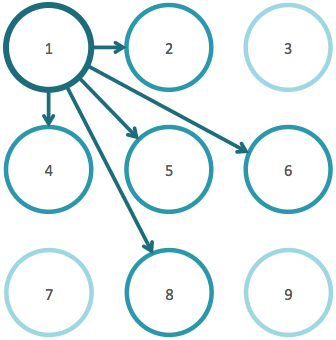
\includegraphics[width=0.4\textwidth]{pics/review/rule1.png}
	      \label{fig:androidrules1}
	    }
	    \hspace{0.8cm}
	    \subfigure[Create a path over a selected node]{
	      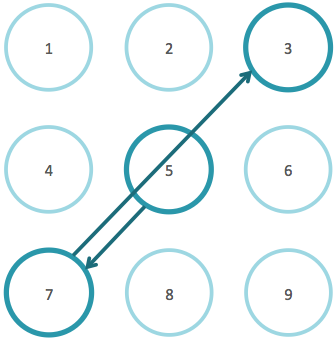
\includegraphics[width=0.4\textwidth]{pics/review/rule2.png}
	      \label{fig:androidrules2}
	    }
	    \caption{Illustration of the Android Pattern creation rules}
	    \label{fig:androidrules}
	  \end{figure}

  In a historical view, the Android Unlock pattern is seen as a new authentication mechanism as opposite to alphanumeric passwords and PIN codes. In a security perspective, the pattern has a total of 389,112 valid patterns using a $3\times3$ grid. Comparing the Android Lock Pattern with PIN codes, having 10.000 possible codes, the Android Lock Pattern seems to be more secure. Compared to an alphanumeric password, the number of combinations depends on the number of characters included. When looking at published research, users are capable of remembering passwords with an average length of 7 to 8 characters. As introduced, the Android unlock pattern is a more suitable form of authentication for mobile devices due to its interactive and graphical form that suits small touch screens. When using an alphanumeric password on a smartphone, a virtual keyboard are used typing the password, making it less suitable for mobile devices because of the size. Smartphones are being used in various situations during a day, making it desirable to use an authentication mechanism that is quick to type and easy to remember, avoid spending the time unlocking the smartphone. It is no secret that an alphanumeric password with its extensive password space would be more secure if users created long passwords. However, this is not the reality because mobile devices do are not suitable for typing long passwords on the virtual keyboard. To further explore the security and usability of the Android unlock pattern,  we will take a look at published research to get an overview.

  	%Table: Number of pattern combinations
	  \begin{table}[H]
	    \centering
	    \begin{tabular}{| l | l |}
	      \hline
	      {\bf \# Length} & {\bf \# Valid combinations} \\ \hline
	      4 & 1624 \\
	      5 & 7152 \\
	      6 & 26,016 \\
	      7 & 72,912 \\
	      8 & 140,704 \\
	      9 & 140,704 \\ \hline
	      Total & 389,112\\ \hline
	    \end{tabular}
	    \caption{Number of pattern combinations}
	    \label{tab:combinations}
	  \end{table}

  As stated, the Android Pattern Lock has 389,112 valid patterns, according to the listed rules. But is this number as secure as it sounds? When looking at the security of a password scheme it can evaluated according to total valid combinations, e.g. the password space or the passwords that statistically are likely of being chosen. The passwords that statistically are likely of being chosen refers to the password space in practice. Table \ref{tab:combinations} summarizes the total number of valid combinations based on the pattern length \cite{Sun}. An another way of look at the security of the a pattern is to measure the pattern strength. A research paper investigated the use of password meter for measuring the strength of a pattern. Their hypothesis was that the utilization of a password meter was providing more secure user-selected patterns. They stated that there often tended to choose a short and easily guessed pattern due to memorability. A password meter is often shown as a colored bar that is often used as an indication of the strength of a password. The research group used a mathematical equation (\ref{eq:patternstrength}) for calculating the strength of Android pattern locks. 

    \begin{equation}\label{eq:patternstrength}
      PS_{P} = S_{P} \times log_{2}(L_{P} + I_{P} + O_{P})
    \end{equation}

  $PS_{p}$ is the strength score of pattern P. $S_{P}$, $L_{P}$, $I_{P}$, and $O_{P}$ are the number of connected nodes, the physical length, the number of intersections, and the number of overlaps of P, respectively. Using Equation \ref{eq:patternstrength} on all valid patterns gives a score from 6.340 to 46.807. The formula was being utilized by Sun et al. \cite{Sun} in their research on Android patterns and password meters. They look at pattern strength in a different way other than just calculating the complexity of a pattern by its length. Calculating password complexity by length seems as a naive approach, making this way more realistic using all the rules of the Android pattern in the equation. When looking at the different characteristics and strength of a pattern used in Equation \ref{eq:patternstrength}, Sun et al. maked distribution graphs of the different characteristics and the strength (Figure \ref{fig:patterngraph}).

  	%Figure: The distribution of the pattern characteristics and strength
    \begin{figure}[H]
      \centering
      \subfigure[Pattern physical length]{
        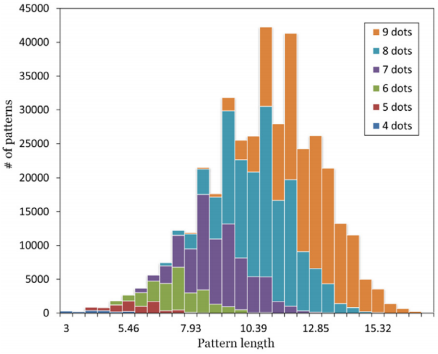
\includegraphics[scale=0.35]{pics/review/patterngraph1}
        \label{fig:patterngraph1}
      }
      \subfigure[Pattern intersections]{
        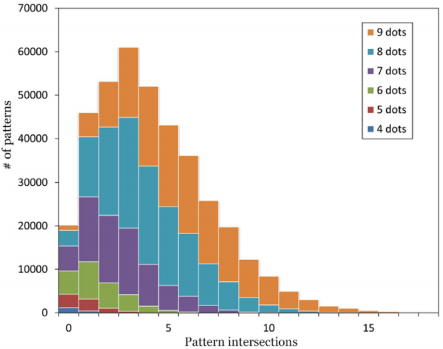
\includegraphics[scale=0.35]{pics/review/patterngraph2}
        \label{fig:patterngraph2}
      }
      \subfigure[Pattern overlaps]{
        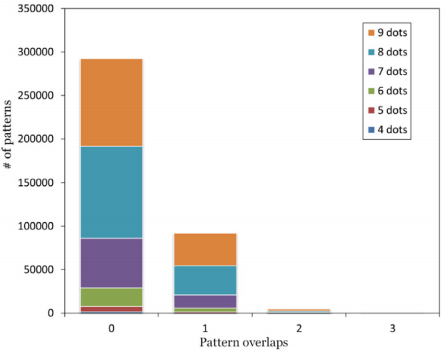
\includegraphics[scale=0.35]{pics/review/patterngraph3}
        \label{fig:patterngraph3}
      }
      \subfigure[Pattern strength]{
        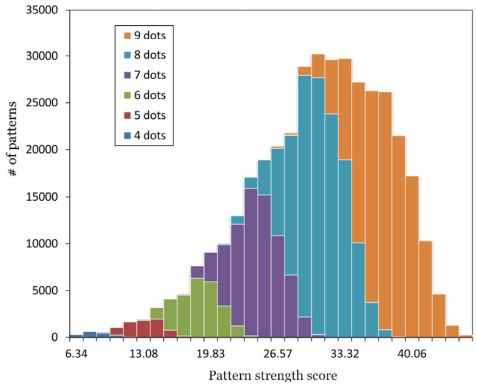
\includegraphics[scale=0.35]{pics/review/patterngraph4}
        \label{fig:patterngraph4}
      }
      \caption{The distribution of the pattern characteristics and strength \cite{Sun}}
      \label{fig:patterngraph}
    \end{figure}

  Sun et al. \cite{Sun} created two different visualizations of a password meter, one looking like a progress bar (Type 1), and one indicating a percent of the strength (Type 2). They recruited 81 participants for a survey testing the strength of user-created patterns. They divided the participants into three separate groups; no password meter (Group A),  password meter type 1 (Group B), and password meter type 2 (Group C). The survey randomly assigned the participants to the separate groups. The result revealed that the strength of the created patterns in group B and C had a higher complexity and strength but had a higher error rate when retyping the pattern. As a researcher explained, users are typically more security conscious when they are aware of the need for such behavior \cite{Sasse}. The error rate points to the problems with passwords and security in general. A long and complicated password are harder to guess but are not likely to be selected due to memorability issues. Also, a problem with the Android Pattern is that the pattern is being frequently used as it is provided to grant access to the smartphone in all kind of situations. The results from the survey states that the input convince was the reason that caused the highest number of participants in the user study not selecting a pattern with a high complexity and strength. A pattern containing more dots takes a longer time to type. When looking at patterns containing intersections and overlaps, there is a high chance of accidentally hitting a wrong dot when drawing a pattern. Such an error are causing the user to redraw the pattern, hence spending more time passing the authentication process. The conclusion is that the time used to type the pattern are as crucial as the time used to memorize the pattern when looking at the users choice in patterns.

  The pattern strength meter gives a score of the visual complexity of a pattern. The benefit of looking at the visual complexity instead of only looking at the length can be seen in Figure \ref{fig:patternstrengthexamples}. When looking at Figure \ref{fig:strength1}, \ref{fig:strength2}, and \ref{fig:strength3}, they have all have the maximum length, but at the same time having a different pattern strength, e.g. a difference in visual complexity. Figure \ref{fig:strength7}, \ref{fig:strength8}, and \ref{fig:strength9} have all the minimum length of four dots, but they still have a difference in the measured strength. The visual complexity is one of the extra security dimensions to study when working with graphical passwords. The pattern itself is just a sequence of numbers, but the order of the sequence can make a big difference in visual complexity, and can be important when wanting to avoid known attacks like shoulder surfing. 

  When looking at user-selected passwords, studies tell that many users are using graphical shapes to support memory \cite{Weiss}. Sun et al. \cite{Sun} analyzed collected Android Lock Patterns and found empirical evidence that some users tended to use patterns which looked like letters or numbers. They found patterns looking like the letters and numbers C, L, N, Z, 2, and 7 that easily can be created on a 3$\times$3 grid. Such a strategy for enhancing memorability by using association elements, e.g something that the user are familiar with, are used in other password schemes. The use of association elements is known to used in PIN codes and alphanumeric passwords where names, objects, dates are used to remember the password instead of a visual representation of a letter or number.

  Android Unlock pattern have been shown to have biases when being user-chosen. A research group did one of the first large-scale user study on the security of the Android Unlock Patterns in order to quantify the security of the {\it Android Pattern Lock} \cite{Uellenbeck}. They analyzed the biases introduced in the pattern making process and added changes to the scheme in order to avoid the known biases in the password scheme. The researchers found that there was a high bias in the pattern selection process, e.g. the upper left corner and three-point long straight lines are likely being selected. If user-chosen patterns were being uniformly chosen, the probability of starting in at any point should be 11\%. The results revealed that there was a strong bias towards the starting point in the corners. If the points were uniformly chosen, the probability for all four corners should be 44\%, but the results showed that the probability is close to 75\% in their pen-and-paper study. In contrast, the center point, the right, the upper, and the lower center points only got a probability of 14\% to be selected. Other results from the pen-and-paper study found that the average pattern length was 5.63 with a standard deviation of 1.5. As stated earlier, users tend to take the easiest way out, making users choose short patterns that are easy to remember and type. Looking at the selection of starting node, 43\% in the user study, and 38\% in the pen-and-paper study selected the upper-left corner as their starting node. This is supporting the researchers claim that users tend to choose less secure patterns ``in the wild'' than a theoretical evaluation of a password scheme.

  What is causing the biases observed in the Android Pattern Lock? The next chapter will introduce a research design for collecting Android Pattern Locks for further analysis focusing on human factors.

  \clearpage

    \begin{figure}[H]
      \centering
      \vspace{1.5cm}
      \subfigure[Sequence: 147852369, \newline Strength: 27.00]{
        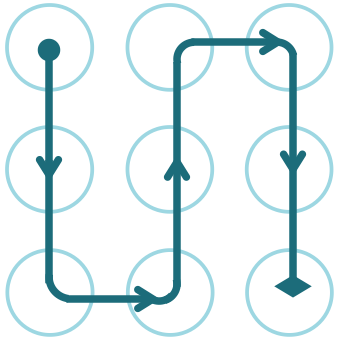
\includegraphics[width=0.27\textwidth]{pics/experiment/strengthpattern2.png}
        \label{fig:strength1}
        \hspace{0.6cm}
      }
      \subfigure[Sequence:213546879, \newline Strength: 36.655]{
        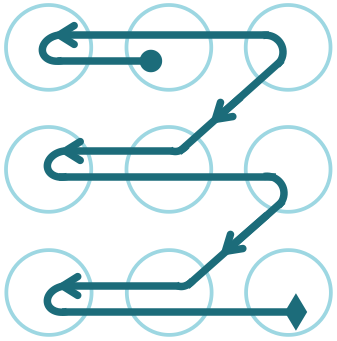
\includegraphics[width=0.27\textwidth]{pics/experiment/strengthpattern3.png}
        \label{fig:strength2}
        \hspace{0.6cm}
      }
      \subfigure[Sequence: 591827346, \newline Strength: 46.807]{
        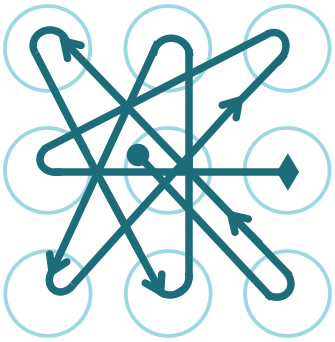
\includegraphics[width=0.27\textwidth]{pics/experiment/strengthpattern1.png}
        \label{fig:strength3}
      }
      \vspace{0.5cm}

      \subfigure[Sequence: 968752, \newline Strength: 15.259]{
        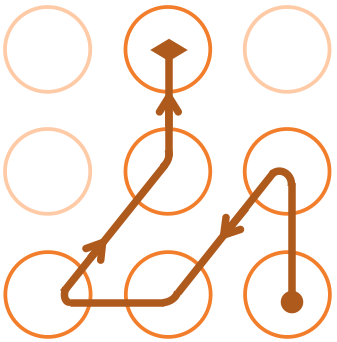
\includegraphics[width=0.27\textwidth]{pics/experiment/strengthpattern7.png}
        \label{fig:strength4}
        \hspace{0.6cm}
      }
      \subfigure[Sequence: 1269853, \newline Strength: 20.781]{
        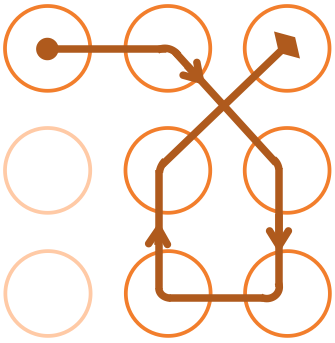
\includegraphics[width=0.27\textwidth]{pics/experiment/strengthpattern8.png}
        \label{fig:strength5}
        \hspace{0.6cm}
      }
      \subfigure[Sequence: 36578249, \newline Strength: 30.512]{
        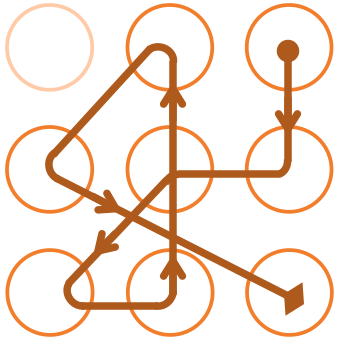
\includegraphics[width=0.27\textwidth]{pics/experiment/strengthpattern9.png}
        \label{fig:strength6}
      }
      
      \vspace{0.5cm}

      \subfigure[Sequence: 1478, \newline Strength: 6.339]{
        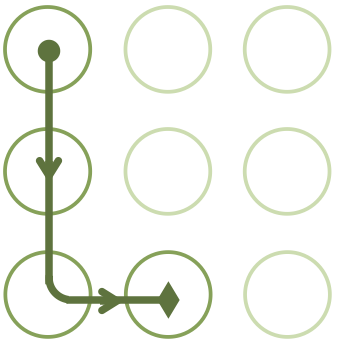
\includegraphics[width=0.27\textwidth]{pics/experiment/strengthpattern4.png}
        \label{fig:strength7}
        \hspace{0.6cm}
      }
      \subfigure[Sequence: 5968, \newline Strength: 9.086]{
        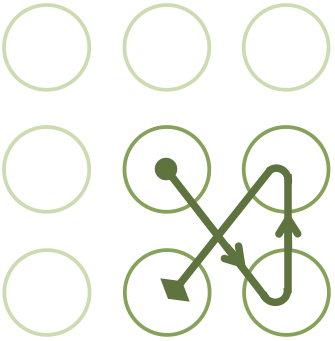
\includegraphics[width=0.27\textwidth]{pics/experiment/strengthpattern5.png}
        \label{fig:strength8}
        \hspace{0.6cm}
      }
      \subfigure[Sequence: 4927, \newline Strength: 11.786]{
        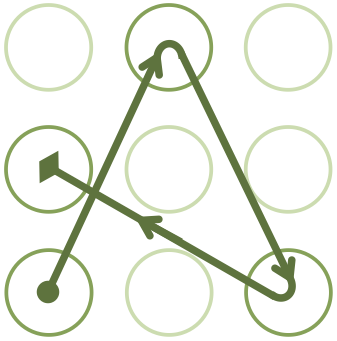
\includegraphics[width=0.27\textwidth]{pics/experiment/strengthpattern6.png}
        \label{fig:strength9}
      }

      \vspace{0.5cm}
      \caption{Examples of patterns with different length and strength}
      \label{fig:patternstrengthexamples}
    \end{figure}
